\documentclass[1p]{elsarticle_modified}
%\bibliographystyle{elsarticle-num}

%\usepackage[colorlinks]{hyperref}
%\usepackage{abbrmath_seonhwa} %\Abb, \Ascr, \Acal ,\Abf, \Afrak
\usepackage{amsfonts}
\usepackage{amssymb}
\usepackage{amsmath}
\usepackage{amsthm}
\usepackage{scalefnt}
\usepackage{amsbsy}
\usepackage{kotex}
\usepackage{caption}
\usepackage{subfig}
\usepackage{color}
\usepackage{graphicx}
\usepackage{xcolor} %% white, black, red, green, blue, cyan, magenta, yellow
\usepackage{float}
\usepackage{setspace}
\usepackage{hyperref}

\usepackage{tikz}
\usetikzlibrary{arrows}

\usepackage{multirow}
\usepackage{array} % fixed length table
\usepackage{hhline}

%%%%%%%%%%%%%%%%%%%%%
\makeatletter
\renewcommand*\env@matrix[1][\arraystretch]{%
	\edef\arraystretch{#1}%
	\hskip -\arraycolsep
	\let\@ifnextchar\new@ifnextchar
	\array{*\c@MaxMatrixCols c}}
\makeatother %https://tex.stackexchange.com/questions/14071/how-can-i-increase-the-line-spacing-in-a-matrix
%%%%%%%%%%%%%%%

\usepackage[normalem]{ulem}

\newcommand{\msout}[1]{\ifmmode\text{\sout{\ensuremath{#1}}}\else\sout{#1}\fi}
%SOURCE: \msout is \stkout macro in https://tex.stackexchange.com/questions/20609/strikeout-in-math-mode

\newcommand{\cancel}[1]{
	\ifmmode
	{\color{red}\msout{#1}}
	\else
	{\color{red}\sout{#1}}
	\fi
}

\newcommand{\add}[1]{
	{\color{blue}\uwave{#1}}
}

\newcommand{\replace}[2]{
	\ifmmode
	{\color{red}\msout{#1}}{\color{blue}\uwave{#2}}
	\else
	{\color{red}\sout{#1}}{\color{blue}\uwave{#2}}
	\fi
}

\newcommand{\Sol}{\mathcal{S}} %segment
\newcommand{\D}{D} %diagram
\newcommand{\A}{\mathcal{A}} %arc


%%%%%%%%%%%%%%%%%%%%%%%%%%%%%5 test

\def\sl{\operatorname{\textup{SL}}(2,\Cbb)}
\def\psl{\operatorname{\textup{PSL}}(2,\Cbb)}
\def\quan{\mkern 1mu \triangleright \mkern 1mu}

\theoremstyle{definition}
\newtheorem{thm}{Theorem}[section]
\newtheorem{prop}[thm]{Proposition}
\newtheorem{lem}[thm]{Lemma}
\newtheorem{ques}[thm]{Question}
\newtheorem{cor}[thm]{Corollary}
\newtheorem{defn}[thm]{Definition}
\newtheorem{exam}[thm]{Example}
\newtheorem{rmk}[thm]{Remark}
\newtheorem{alg}[thm]{Algorithm}

\newcommand{\I}{\sqrt{-1}}
\begin{document}

%\begin{frontmatter}
%
%\title{Boundary parabolic representations of knots up to 8 crossings}
%
%%% Group authors per affiliation:
%\author{Yunhi Cho} 
%\address{Department of Mathematics, University of Seoul, Seoul, Korea}
%\ead{yhcho@uos.ac.kr}
%
%
%\author{Seonhwa Kim} %\fnref{s_kim}}
%\address{Center for Geometry and Physics, Institute for Basic Science, Pohang, 37673, Korea}
%\ead{ryeona17@ibs.re.kr}
%
%\author{Hyuk Kim}
%\address{Department of Mathematical Sciences, Seoul National University, Seoul 08826, Korea}
%\ead{hyukkim@snu.ac.kr}
%
%\author{Seokbeom Yoon}
%\address{Department of Mathematical Sciences, Seoul National University, Seoul, 08826,  Korea}
%\ead{sbyoon15@snu.ac.kr}
%
%\begin{abstract}
%We find all boundary parabolic representation of knots up to 8 crossings.
%
%\end{abstract}
%\begin{keyword}
%    \MSC[2010] 57M25 
%\end{keyword}
%
%\end{frontmatter}

%\linenumbers
%\tableofcontents
%
\newcommand\colored[1]{\textcolor{white}{\rule[-0.35ex]{0.8em}{1.4ex}}\kern-0.8em\color{red} #1}%
%\newcommand\colored[1]{\textcolor{white}{ #1}\kern-2.17ex	\textcolor{white}{ #1}\kern-1.81ex	\textcolor{white}{ #1}\kern-2.15ex\color{red}#1	}

{\Large $\underline{12a_{0883}~(K12a_{0883})}$}

\setlength{\tabcolsep}{10pt}
\renewcommand{\arraystretch}{1.6}
\vspace{1cm}\begin{tabular}{m{100pt}>{\centering\arraybackslash}m{274pt}}
\multirow{5}{120pt}{
	\centering
	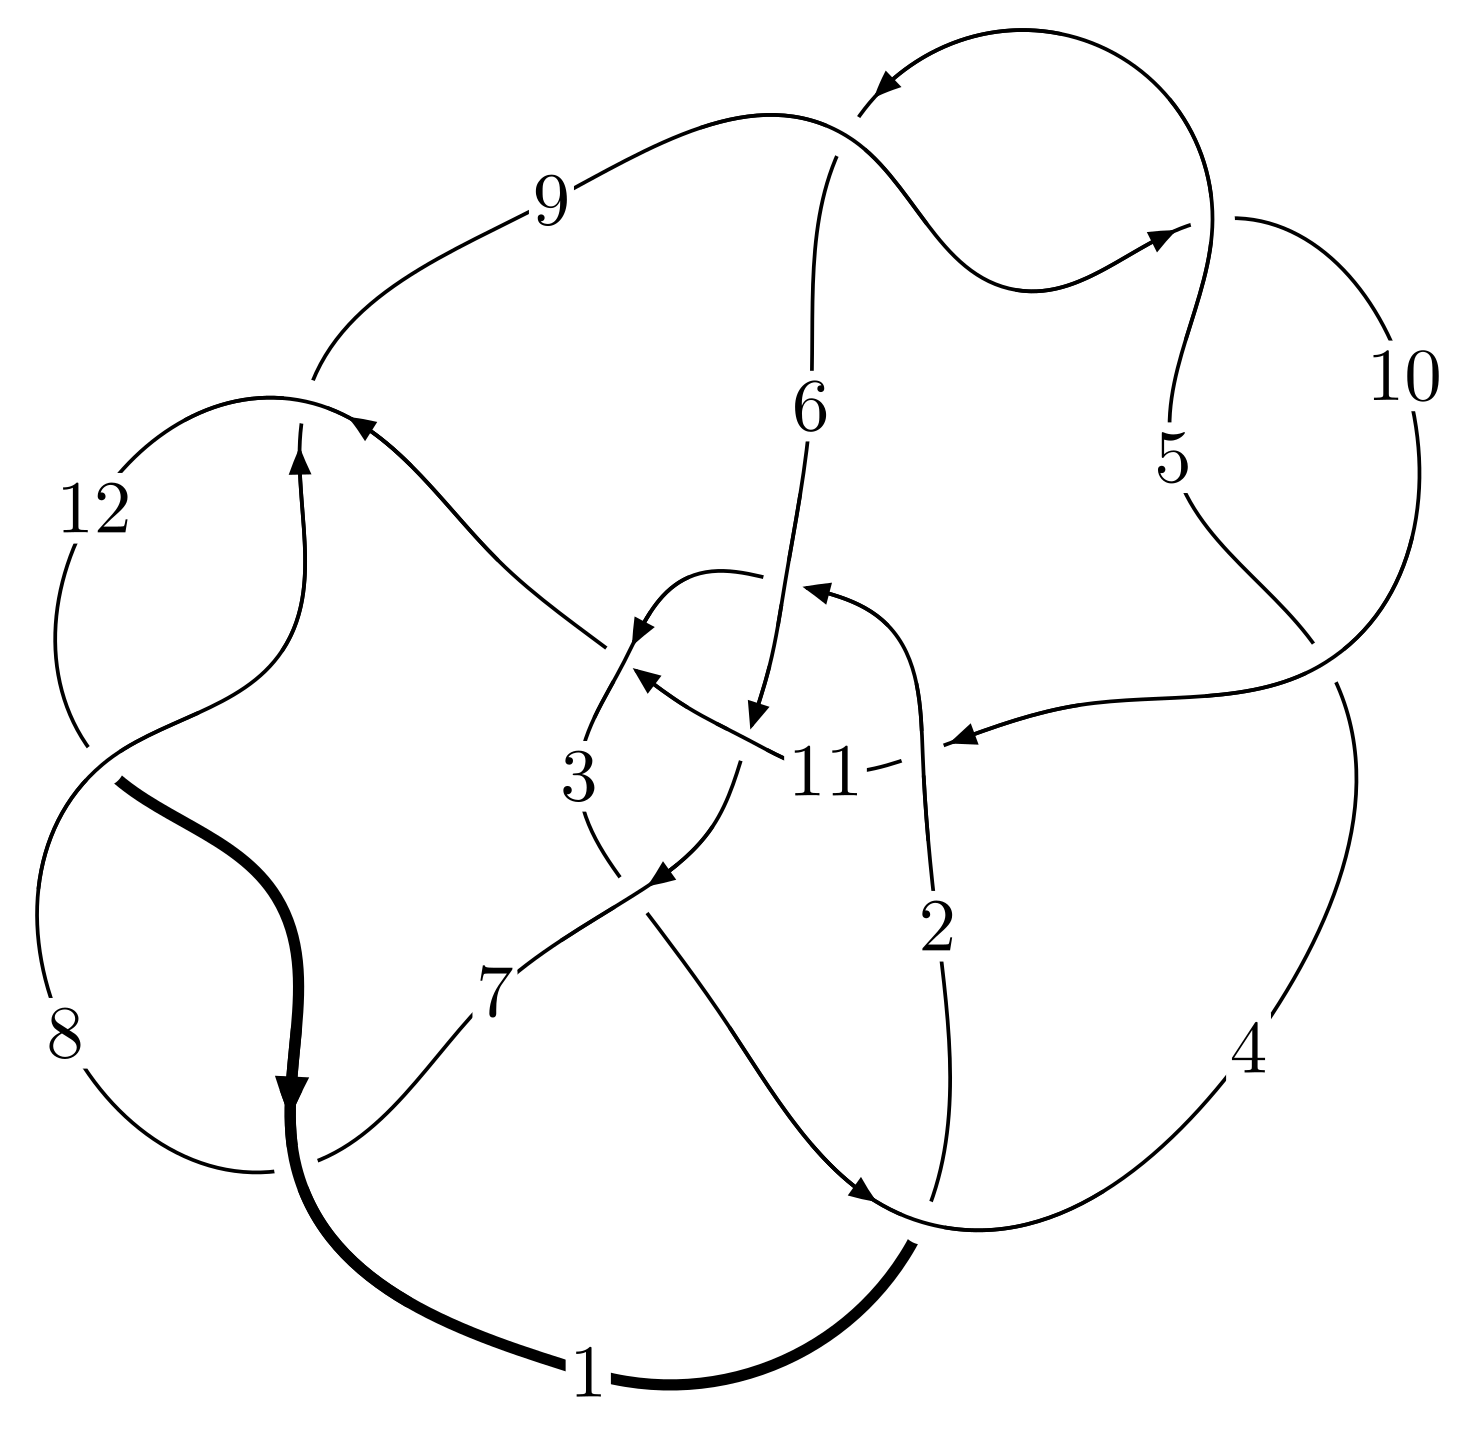
\includegraphics[width=112pt]{../../../GIT/diagram.site/Diagrams/png/1684_12a_0883.png}\\
\ \ \ A knot diagram\footnotemark}&
\allowdisplaybreaks
\textbf{Linearized knot diagam} \\
\cline{2-2}
 &
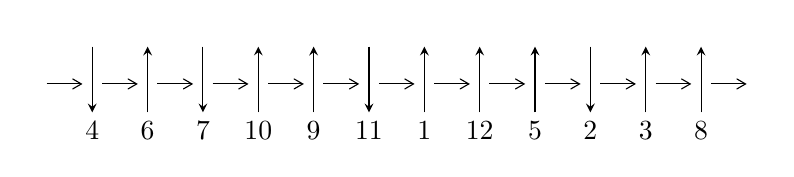
\begin{tikzpicture}[x=20pt, y=17pt]
	% nodes
	\node (C0) at (0, 0) {};
	\node (C1) at (1, 0) {};
	\node (C1U) at (1, +1) {};
	\node (C1D) at (1, -1) {4};

	\node (C2) at (2, 0) {};
	\node (C2U) at (2, +1) {};
	\node (C2D) at (2, -1) {6};

	\node (C3) at (3, 0) {};
	\node (C3U) at (3, +1) {};
	\node (C3D) at (3, -1) {7};

	\node (C4) at (4, 0) {};
	\node (C4U) at (4, +1) {};
	\node (C4D) at (4, -1) {10};

	\node (C5) at (5, 0) {};
	\node (C5U) at (5, +1) {};
	\node (C5D) at (5, -1) {9};

	\node (C6) at (6, 0) {};
	\node (C6U) at (6, +1) {};
	\node (C6D) at (6, -1) {11};

	\node (C7) at (7, 0) {};
	\node (C7U) at (7, +1) {};
	\node (C7D) at (7, -1) {1};

	\node (C8) at (8, 0) {};
	\node (C8U) at (8, +1) {};
	\node (C8D) at (8, -1) {12};

	\node (C9) at (9, 0) {};
	\node (C9U) at (9, +1) {};
	\node (C9D) at (9, -1) {5};

	\node (C10) at (10, 0) {};
	\node (C10U) at (10, +1) {};
	\node (C10D) at (10, -1) {2};

	\node (C11) at (11, 0) {};
	\node (C11U) at (11, +1) {};
	\node (C11D) at (11, -1) {3};

	\node (C12) at (12, 0) {};
	\node (C12U) at (12, +1) {};
	\node (C12D) at (12, -1) {8};
	\node (C13) at (13, 0) {};

	% arrows
	\draw[->,>={angle 60}]
	(C0) edge (C1) (C1) edge (C2) (C2) edge (C3) (C3) edge (C4) (C4) edge (C5) (C5) edge (C6) (C6) edge (C7) (C7) edge (C8) (C8) edge (C9) (C9) edge (C10) (C10) edge (C11) (C11) edge (C12) (C12) edge (C13) ;	\draw[->,>=stealth]
	(C1U) edge (C1D) (C2D) edge (C2U) (C3U) edge (C3D) (C4D) edge (C4U) (C5D) edge (C5U) (C6U) edge (C6D) (C7D) edge (C7U) (C8D) edge (C8U) (C9D) edge (C9U) (C10U) edge (C10D) (C11D) edge (C11U) (C12D) edge (C12U) ;
	\end{tikzpicture} \\
\hhline{~~} \\& 
\textbf{Solving Sequence} \\ \cline{2-2} 
 &
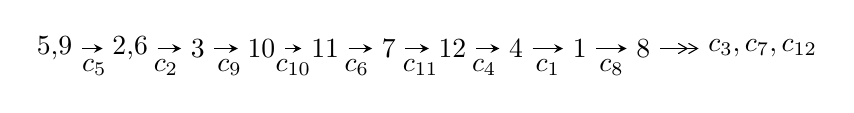
\begin{tikzpicture}[x=23pt, y=7pt]
	% node
	\node (A0) at (-1/8, 0) {5,9};
	\node (A1) at (17/16, 0) {2,6};
	\node (A2) at (17/8, 0) {3};
	\node (A3) at (25/8, 0) {10};
	\node (A4) at (33/8, 0) {11};
	\node (A5) at (41/8, 0) {7};
	\node (A6) at (49/8, 0) {12};
	\node (A7) at (57/8, 0) {4};
	\node (A8) at (65/8, 0) {1};
	\node (A9) at (73/8, 0) {8};
	\node (C1) at (1/2, -1) {$c_{5}$};
	\node (C2) at (13/8, -1) {$c_{2}$};
	\node (C3) at (21/8, -1) {$c_{9}$};
	\node (C4) at (29/8, -1) {$c_{10}$};
	\node (C5) at (37/8, -1) {$c_{6}$};
	\node (C6) at (45/8, -1) {$c_{11}$};
	\node (C7) at (53/8, -1) {$c_{4}$};
	\node (C8) at (61/8, -1) {$c_{1}$};
	\node (C9) at (69/8, -1) {$c_{8}$};
	\node (A10) at (11, 0) {$c_{3},c_{7},c_{12}$};

	% edge
	\draw[->,>=stealth]	
	(A0) edge (A1) (A1) edge (A2) (A2) edge (A3) (A3) edge (A4) (A4) edge (A5) (A5) edge (A6) (A6) edge (A7) (A7) edge (A8) (A8) edge (A9) ;
	\draw[->>,>={angle 60}]	
	(A9) edge (A10);
\end{tikzpicture} \\ 

\end{tabular} \\

\footnotetext{
The image of knot diagram is generated by the software ``\textbf{Draw programme}" developed by Andrew Bartholomew(\url{http://www.layer8.co.uk/maths/draw/index.htm\#Running-draw}), where we modified some parts for our purpose(\url{https://github.com/CATsTAILs/LinksPainter}).
}\phantom \\ \newline 
\centering \textbf{Ideals for irreducible components\footnotemark of $X_{\text{par}}$} 
 
\begin{align*}
I^u_{1}&=\langle 
161211550 u^{26}+163067087 u^{25}+\cdots+168567233 b+184311963,\\
\phantom{I^u_{1}}&\phantom{= \langle  }-64532319 u^{26}-105037379 u^{25}+\cdots+168567233 a-400814896,\;u^{27}+u^{26}+\cdots+2 u-1\rangle \\
I^u_{2}&=\langle 
8.05343\times10^{231} u^{97}-2.98534\times10^{231} u^{96}+\cdots+7.84596\times10^{231} b-9.54856\times10^{232},\\
\phantom{I^u_{2}}&\phantom{= \langle  }1.36459\times10^{233} u^{97}-1.17790\times10^{233} u^{96}+\cdots+7.84596\times10^{231} a-1.42631\times10^{234},\;u^{98}- u^{97}+\cdots-36 u+1\rangle \\
I^u_{3}&=\langle 
u^4+u^3+2 u^2+b+2 u,\;- u^6-2 u^4- u^3+u^2+a- u+1,\;u^7+u^6+4 u^5+5 u^4+5 u^3+6 u^2+2 u+1\rangle \\
I^u_{4}&=\langle 
4 u^{25}-11 u^{24}+\cdots+b-3,\;5 u^{25}-13 u^{24}+\cdots+a+4,\;u^{26}-2 u^{25}+\cdots-2 u+1\rangle \\
\\
\end{align*}
\raggedright * 4 irreducible components of $\dim_{\mathbb{C}}=0$, with total 158 representations.\\
\footnotetext{All coefficients of polynomials are rational numbers. But the coefficients are sometimes approximated in decimal forms when there is not enough margin.}
\newpage
\renewcommand{\arraystretch}{1}
\centering \section*{I. $I^u_{1}= \langle 1.61\times10^{8} u^{26}+1.63\times10^{8} u^{25}+\cdots+1.69\times10^{8} b+1.84\times10^{8},\;-6.45\times10^{7} u^{26}-1.05\times10^{8} u^{25}+\cdots+1.69\times10^{8} a-4.01\times10^{8},\;u^{27}+u^{26}+\cdots+2 u-1 \rangle$}
\flushleft \textbf{(i) Arc colorings}\\
\begin{tabular}{m{7pt} m{180pt} m{7pt} m{180pt} }
\flushright $a_{5}=$&$\begin{pmatrix}1\\0\end{pmatrix}$ \\
\flushright $a_{9}=$&$\begin{pmatrix}0\\u\end{pmatrix}$ \\
\flushright $a_{2}=$&$\begin{pmatrix}0.382828 u^{26}+0.623119 u^{25}+\cdots+2.47957 u+2.37777\\-0.956364 u^{26}-0.967371 u^{25}+\cdots-0.798674 u-1.09340\end{pmatrix}$ \\
\flushright $a_{6}=$&$\begin{pmatrix}1\\- u^2\end{pmatrix}$ \\
\flushright $a_{3}=$&$\begin{pmatrix}0.110178 u^{26}+0.0591229 u^{25}+\cdots+1.58315 u+1.52466\\-0.538924 u^{26}-0.745833 u^{25}+\cdots-1.10871 u-0.802058\end{pmatrix}$ \\
\flushright $a_{10}=$&$\begin{pmatrix}u\\u\end{pmatrix}$ \\
\flushright $a_{11}=$&$\begin{pmatrix}-0.959060 u^{26}-1.36051 u^{25}+\cdots+0.0254923 u-2.73531\\-0.00114729 u^{26}+0.449549 u^{25}+\cdots+1.51778 u+0.626626\end{pmatrix}$ \\
\flushright $a_{7}=$&$\begin{pmatrix}- u^3-2 u\\0.576586 u^{26}+1.01727 u^{25}+\cdots+1.09757 u+0.898510\end{pmatrix}$ \\
\flushright $a_{12}=$&$\begin{pmatrix}-1\\0.469768 u^{26}+0.828129 u^{25}+\cdots+1.88993 u+0.768115\end{pmatrix}$ \\
\flushright $a_{4}=$&$\begin{pmatrix}u^2+1\\u^2\end{pmatrix}$ \\
\flushright $a_{1}=$&$\begin{pmatrix}u^2+1\\-0.428742 u^{26}-0.646967 u^{25}+\cdots-1.64298 u-1.12648\end{pmatrix}$ \\
\flushright $a_{8}=$&$\begin{pmatrix}- u\\0.358361 u^{26}+0.317336 u^{25}+\cdots+0.828580 u+0.469768\end{pmatrix}$\\&\end{tabular}
\flushleft \textbf{(ii) Obstruction class $= -1$}\\~\\
\flushleft \textbf{(iii) Cusp Shapes $= -\frac{314978218}{168567233} u^{26}-\frac{605025497}{168567233} u^{25}+\cdots-\frac{1917677278}{168567233} u+\frac{586286315}{168567233}$}\\~\\
\newpage\renewcommand{\arraystretch}{1}
\flushleft \textbf{(iv) u-Polynomials at the component}\newline \\
\begin{tabular}{m{50pt}|m{274pt}}
Crossings & \hspace{64pt}u-Polynomials at each crossing \\
\hline $$\begin{aligned}c_{1}\end{aligned}$$&$\begin{aligned}
&u^{27}-7 u^{26}+\cdots+176 u-16
\end{aligned}$\\
\hline $$\begin{aligned}c_{2},c_{11}\end{aligned}$$&$\begin{aligned}
&u^{27}+u^{26}+\cdots-3 u+1
\end{aligned}$\\
\hline $$\begin{aligned}c_{3},c_{10}\end{aligned}$$&$\begin{aligned}
&u^{27}+u^{26}+\cdots+3 u+1
\end{aligned}$\\
\hline $$\begin{aligned}c_{4},c_{5},c_{7}\\c_{8},c_{9},c_{12}\end{aligned}$$&$\begin{aligned}
&u^{27}- u^{26}+\cdots+2 u+1
\end{aligned}$\\
\hline $$\begin{aligned}c_{6}\end{aligned}$$&$\begin{aligned}
&u^{27}-16 u^{26}+\cdots+22 u-4
\end{aligned}$\\
\hline
\end{tabular}\\~\\
\newpage\renewcommand{\arraystretch}{1}
\flushleft \textbf{(v) Riley Polynomials at the component}\newline \\
\begin{tabular}{m{50pt}|m{274pt}}
Crossings & \hspace{64pt}Riley Polynomials at each crossing \\
\hline $$\begin{aligned}c_{1}\end{aligned}$$&$\begin{aligned}
&y^{27}-5 y^{26}+\cdots+5280 y-256
\end{aligned}$\\
\hline $$\begin{aligned}c_{2},c_{11}\end{aligned}$$&$\begin{aligned}
&y^{27}-7 y^{26}+\cdots+27 y-1
\end{aligned}$\\
\hline $$\begin{aligned}c_{3},c_{10}\end{aligned}$$&$\begin{aligned}
&y^{27}-7 y^{26}+\cdots+17 y-1
\end{aligned}$\\
\hline $$\begin{aligned}c_{4},c_{5},c_{7}\\c_{8},c_{9},c_{12}\end{aligned}$$&$\begin{aligned}
&y^{27}+25 y^{26}+\cdots+18 y-1
\end{aligned}$\\
\hline $$\begin{aligned}c_{6}\end{aligned}$$&$\begin{aligned}
&y^{27}-10 y^{26}+\cdots+492 y-16
\end{aligned}$\\
\hline
\end{tabular}\\~\\
\newpage\flushleft \textbf{(vi) Complex Volumes and Cusp Shapes}
$$\begin{array}{c|c|c}  
\text{Solutions to }I^u_{1}& \I (\text{vol} + \sqrt{-1}CS) & \text{Cusp shape}\\
 \hline 
\begin{aligned}
u &= \phantom{-}0.070166 + 0.997411 I \\
a &= \phantom{-}0.050375 + 0.136338 I \\
b &= \phantom{-}1.106230 + 0.535575 I\end{aligned}
 & -0.70818 + 3.60837 I & \phantom{-}2.50627 - 4.79457 I \\ \hline\begin{aligned}
u &= \phantom{-}0.070166 - 0.997411 I \\
a &= \phantom{-}0.050375 - 0.136338 I \\
b &= \phantom{-}1.106230 - 0.535575 I\end{aligned}
 & -0.70818 - 3.60837 I & \phantom{-}2.50627 + 4.79457 I \\ \hline\begin{aligned}
u &= -0.995972 + 0.202368 I \\
a &= -0.0990140 + 0.0471163 I \\
b &= \phantom{-}0.473624 + 0.134565 I\end{aligned}
 & -0.0498204 + 0.0658137 I & \phantom{-}13.3792 - 20.3584 I \\ \hline\begin{aligned}
u &= -0.995972 - 0.202368 I \\
a &= -0.0990140 - 0.0471163 I \\
b &= \phantom{-}0.473624 - 0.134565 I\end{aligned}
 & -0.0498204 - 0.0658137 I & \phantom{-}13.3792 + 20.3584 I \\ \hline\begin{aligned}
u &= \phantom{-}0.791226 + 0.513863 I \\
a &= -0.736086 + 0.718981 I \\
b &= -0.141477 - 0.624312 I\end{aligned}
 & -1.14567 + 9.89138 I & \phantom{-}2.32394 - 9.56251 I \\ \hline\begin{aligned}
u &= \phantom{-}0.791226 - 0.513863 I \\
a &= -0.736086 - 0.718981 I \\
b &= -0.141477 + 0.624312 I\end{aligned}
 & -1.14567 - 9.89138 I & \phantom{-}2.32394 + 9.56251 I \\ \hline\begin{aligned}
u &= -0.542866 + 0.539927 I \\
a &= \phantom{-}0.390658 - 0.702555 I \\
b &= -0.0570518 + 0.0874559 I\end{aligned}
 & \phantom{-}1.32847 - 1.67905 I & \phantom{-}10.52150 + 4.30869 I \\ \hline\begin{aligned}
u &= -0.542866 - 0.539927 I \\
a &= \phantom{-}0.390658 + 0.702555 I \\
b &= -0.0570518 - 0.0874559 I\end{aligned}
 & \phantom{-}1.32847 + 1.67905 I & \phantom{-}10.52150 - 4.30869 I \\ \hline\begin{aligned}
u &= -0.122477 + 1.262950 I \\
a &= -1.31674 - 1.34075 I \\
b &= -1.11217 - 2.28394 I\end{aligned}
 & -9.69201 - 3.22381 I & -6.38040 + 1.87892 I \\ \hline\begin{aligned}
u &= -0.122477 - 1.262950 I \\
a &= -1.31674 + 1.34075 I \\
b &= -1.11217 + 2.28394 I\end{aligned}
 & -9.69201 + 3.22381 I & -6.38040 - 1.87892 I\\
 \hline 
 \end{array}$$\newpage$$\begin{array}{c|c|c}  
\text{Solutions to }I^u_{1}& \I (\text{vol} + \sqrt{-1}CS) & \text{Cusp shape}\\
 \hline 
\begin{aligned}
u &= \phantom{-}0.230598 + 1.267870 I \\
a &= -0.39953 + 1.81101 I \\
b &= -0.47291 + 2.86023 I\end{aligned}
 & -7.30514 + 6.01759 I & -0.32733 - 7.30981 I \\ \hline\begin{aligned}
u &= \phantom{-}0.230598 - 1.267870 I \\
a &= -0.39953 - 1.81101 I \\
b &= -0.47291 - 2.86023 I\end{aligned}
 & -7.30514 - 6.01759 I & -0.32733 + 7.30981 I \\ \hline\begin{aligned}
u &= \phantom{-}0.204690 + 1.330900 I \\
a &= -0.26598 + 1.62179 I \\
b &= -0.47881 + 1.96936 I\end{aligned}
 & -7.82612 + 5.05552 I & -1.17987 - 2.39455 I \\ \hline\begin{aligned}
u &= \phantom{-}0.204690 - 1.330900 I \\
a &= -0.26598 - 1.62179 I \\
b &= -0.47881 - 1.96936 I\end{aligned}
 & -7.82612 - 5.05552 I & -1.17987 + 2.39455 I \\ \hline\begin{aligned}
u &= -0.179338 + 1.344090 I \\
a &= -0.04177 - 2.74708 I \\
b &= \phantom{-}0.38158 - 3.28794 I\end{aligned}
 & -8.31053 - 8.16537 I & -3.33517 + 11.01444 I \\ \hline\begin{aligned}
u &= -0.179338 - 1.344090 I \\
a &= -0.04177 + 2.74708 I \\
b &= \phantom{-}0.38158 + 3.28794 I\end{aligned}
 & -8.31053 + 8.16537 I & -3.33517 - 11.01444 I \\ \hline\begin{aligned}
u &= -0.603103\phantom{ +0.000000I} \\
a &= \phantom{-}2.07379\phantom{ +0.000000I} \\
b &= \phantom{-}0.171319\phantom{ +0.000000I}\end{aligned}
 & \phantom{-}0.515822\phantom{ +0.000000I} & \phantom{-}11.7560\phantom{ +0.000000I} \\ \hline\begin{aligned}
u &= \phantom{-}0.01958 + 1.42133 I \\
a &= \phantom{-}0.704503 + 0.398347 I \\
b &= -0.235482 + 0.318924 I\end{aligned}
 & -6.81655 + 2.85614 I & -2.29662 - 2.94714 I \\ \hline\begin{aligned}
u &= \phantom{-}0.01958 - 1.42133 I \\
a &= \phantom{-}0.704503 - 0.398347 I \\
b &= -0.235482 - 0.318924 I\end{aligned}
 & -6.81655 - 2.85614 I & -2.29662 + 2.94714 I \\ \hline\begin{aligned}
u &= -0.473384\phantom{ +0.000000I} \\
a &= \phantom{-}1.02334\phantom{ +0.000000I} \\
b &= \phantom{-}0.321318\phantom{ +0.000000I}\end{aligned}
 & \phantom{-}0.921050\phantom{ +0.000000I} & \phantom{-}10.8530\phantom{ +0.000000I}\\
 \hline 
 \end{array}$$\newpage$$\begin{array}{c|c|c}  
\text{Solutions to }I^u_{1}& \I (\text{vol} + \sqrt{-1}CS) & \text{Cusp shape}\\
 \hline 
\begin{aligned}
u &= \phantom{-}0.375751 + 0.179645 I \\
a &= \phantom{-}0.80850 - 1.25731 I \\
b &= \phantom{-}0.727471 + 0.972773 I\end{aligned}
 & \phantom{-}1.25767 + 3.71987 I & \phantom{-}13.1792 - 10.4060 I \\ \hline\begin{aligned}
u &= \phantom{-}0.375751 - 0.179645 I \\
a &= \phantom{-}0.80850 + 1.25731 I \\
b &= \phantom{-}0.727471 - 0.972773 I\end{aligned}
 & \phantom{-}1.25767 - 3.71987 I & \phantom{-}13.1792 + 10.4060 I \\ \hline\begin{aligned}
u &= -0.32805 + 1.55024 I \\
a &= \phantom{-}0.08115 + 1.75485 I \\
b &= -0.33517 + 2.81280 I\end{aligned}
 & -14.5174 - 18.3439 I & -3.23925 + 8.58445 I \\ \hline\begin{aligned}
u &= -0.32805 - 1.55024 I \\
a &= \phantom{-}0.08115 - 1.75485 I \\
b &= -0.33517 - 2.81280 I\end{aligned}
 & -14.5174 + 18.3439 I & -3.23925 - 8.58445 I \\ \hline\begin{aligned}
u &= \phantom{-}0.35424 + 1.56608 I \\
a &= \phantom{-}0.129600 - 1.020350 I \\
b &= -0.22137 - 1.77783 I\end{aligned}
 & -13.3669 + 10.0927 I & -3.30444 - 7.62979 I \\ \hline\begin{aligned}
u &= \phantom{-}0.35424 - 1.56608 I \\
a &= \phantom{-}0.129600 + 1.020350 I \\
b &= -0.22137 + 1.77783 I\end{aligned}
 & -13.3669 - 10.0927 I & -3.30444 + 7.62979 I \\ \hline\begin{aligned}
u &= \phantom{-}0.321408\phantom{ +0.000000I} \\
a &= \phantom{-}2.29153\phantom{ +0.000000I} \\
b &= -0.761575\phantom{ +0.000000I}\end{aligned}
 & -2.01710\phantom{ +0.000000I} & -4.30310\phantom{ +0.000000I}\\
 \hline 
 \end{array}$$\newpage\newpage\renewcommand{\arraystretch}{1}
\centering \section*{II. $I^u_{2}= \langle 8.05\times10^{231} u^{97}-2.99\times10^{231} u^{96}+\cdots+7.85\times10^{231} b-9.55\times10^{232},\;1.36\times10^{233} u^{97}-1.18\times10^{233} u^{96}+\cdots+7.85\times10^{231} a-1.43\times10^{234},\;u^{98}- u^{97}+\cdots-36 u+1 \rangle$}
\flushleft \textbf{(i) Arc colorings}\\
\begin{tabular}{m{7pt} m{180pt} m{7pt} m{180pt} }
\flushright $a_{5}=$&$\begin{pmatrix}1\\0\end{pmatrix}$ \\
\flushright $a_{9}=$&$\begin{pmatrix}0\\u\end{pmatrix}$ \\
\flushright $a_{2}=$&$\begin{pmatrix}-17.3923 u^{97}+15.0129 u^{96}+\cdots-4433.65 u+181.789\\-1.02644 u^{97}+0.380494 u^{96}+\cdots-235.466 u+12.1700\end{pmatrix}$ \\
\flushright $a_{6}=$&$\begin{pmatrix}1\\- u^2\end{pmatrix}$ \\
\flushright $a_{3}=$&$\begin{pmatrix}-17.9778 u^{97}+15.8292 u^{96}+\cdots-4737.38 u+196.338\\-0.273211 u^{97}+0.251929 u^{96}+\cdots-244.360 u+12.4008\end{pmatrix}$ \\
\flushright $a_{10}=$&$\begin{pmatrix}u\\u\end{pmatrix}$ \\
\flushright $a_{11}=$&$\begin{pmatrix}-9.95056 u^{97}+8.64388 u^{96}+\cdots-2431.59 u+104.303\\0.850940 u^{97}-0.650011 u^{96}+\cdots+280.898 u-11.5019\end{pmatrix}$ \\
\flushright $a_{7}=$&$\begin{pmatrix}-4.56522 u^{97}+3.03576 u^{96}+\cdots-694.079 u+32.8371\\1.99051 u^{97}-2.57908 u^{96}+\cdots+546.222 u-22.8070\end{pmatrix}$ \\
\flushright $a_{12}=$&$\begin{pmatrix}-24.0010 u^{97}+22.2667 u^{96}+\cdots-7216.77 u+308.025\\-1.43913 u^{97}+1.65677 u^{96}+\cdots-365.233 u+18.0341\end{pmatrix}$ \\
\flushright $a_{4}=$&$\begin{pmatrix}u^2+1\\u^2\end{pmatrix}$ \\
\flushright $a_{1}=$&$\begin{pmatrix}-17.4547 u^{97}+15.3237 u^{96}+\cdots-4630.14 u+192.443\\-0.306071 u^{97}+0.126649 u^{96}+\cdots-242.535 u+12.3881\end{pmatrix}$ \\
\flushright $a_{8}=$&$\begin{pmatrix}-2.91621 u^{97}+2.48251 u^{96}+\cdots-1005.31 u+66.4486\\4.29285 u^{97}-4.18123 u^{96}+\cdots+1267.97 u-52.9233\end{pmatrix}$\\&\end{tabular}
\flushleft \textbf{(ii) Obstruction class $= -1$}\\~\\
\flushleft \textbf{(iii) Cusp Shapes $= -6.62974 u^{97}+5.53191 u^{96}+\cdots-803.454 u+33.3318$}\\~\\
\newpage\renewcommand{\arraystretch}{1}
\flushleft \textbf{(iv) u-Polynomials at the component}\newline \\
\begin{tabular}{m{50pt}|m{274pt}}
Crossings & \hspace{64pt}u-Polynomials at each crossing \\
\hline $$\begin{aligned}c_{1}\end{aligned}$$&$\begin{aligned}
&(u^{49}+8 u^{48}+\cdots- u+139)^{2}
\end{aligned}$\\
\hline $$\begin{aligned}c_{2},c_{11}\end{aligned}$$&$\begin{aligned}
&u^{98}- u^{97}+\cdots+78991 u+5641
\end{aligned}$\\
\hline $$\begin{aligned}c_{3},c_{10}\end{aligned}$$&$\begin{aligned}
&u^{98}-12 u^{96}+\cdots-2731098 u+1190927
\end{aligned}$\\
\hline $$\begin{aligned}c_{4},c_{5},c_{7}\\c_{8},c_{9},c_{12}\end{aligned}$$&$\begin{aligned}
&u^{98}+u^{97}+\cdots+36 u+1
\end{aligned}$\\
\hline $$\begin{aligned}c_{6}\end{aligned}$$&$\begin{aligned}
&(u^{49}+6 u^{48}+\cdots+7 u+1)^{2}
\end{aligned}$\\
\hline
\end{tabular}\\~\\
\newpage\renewcommand{\arraystretch}{1}
\flushleft \textbf{(v) Riley Polynomials at the component}\newline \\
\begin{tabular}{m{50pt}|m{274pt}}
Crossings & \hspace{64pt}Riley Polynomials at each crossing \\
\hline $$\begin{aligned}c_{1}\end{aligned}$$&$\begin{aligned}
&(y^{49}-30 y^{48}+\cdots-378913 y-19321)^{2}
\end{aligned}$\\
\hline $$\begin{aligned}c_{2},c_{11}\end{aligned}$$&$\begin{aligned}
&y^{98}+23 y^{97}+\cdots+672079733 y+31820881
\end{aligned}$\\
\hline $$\begin{aligned}c_{3},c_{10}\end{aligned}$$&$\begin{aligned}
&y^{98}-24 y^{97}+\cdots-54241979206882 y+1418307119329
\end{aligned}$\\
\hline $$\begin{aligned}c_{4},c_{5},c_{7}\\c_{8},c_{9},c_{12}\end{aligned}$$&$\begin{aligned}
&y^{98}+101 y^{97}+\cdots-326 y+1
\end{aligned}$\\
\hline $$\begin{aligned}c_{6}\end{aligned}$$&$\begin{aligned}
&(y^{49}-6 y^{48}+\cdots+25 y-1)^{2}
\end{aligned}$\\
\hline
\end{tabular}\\~\\
\newpage\flushleft \textbf{(vi) Complex Volumes and Cusp Shapes}
$$\begin{array}{c|c|c}  
\text{Solutions to }I^u_{2}& \I (\text{vol} + \sqrt{-1}CS) & \text{Cusp shape}\\
 \hline 
\begin{aligned}
u &= -0.601265 + 0.799530 I \\
a &= \phantom{-}0.371144 + 0.018717 I \\
b &= \phantom{-}0.411619 - 0.292634 I\end{aligned}
 & \phantom{-}0.89188 - 2.50997 I & \phantom{-0.000000 } 0 \\ \hline\begin{aligned}
u &= -0.601265 - 0.799530 I \\
a &= \phantom{-}0.371144 - 0.018717 I \\
b &= \phantom{-}0.411619 + 0.292634 I\end{aligned}
 & \phantom{-}0.89188 + 2.50997 I & \phantom{-0.000000 } 0 \\ \hline\begin{aligned}
u &= \phantom{-}0.742965 + 0.599497 I \\
a &= -0.341644 - 0.232431 I \\
b &= \phantom{-}0.575289 - 0.479550 I\end{aligned}
 & -1.41187 - 4.73118 I & \phantom{-0.000000 } 0 \\ \hline\begin{aligned}
u &= \phantom{-}0.742965 - 0.599497 I \\
a &= -0.341644 + 0.232431 I \\
b &= \phantom{-}0.575289 + 0.479550 I\end{aligned}
 & -1.41187 + 4.73118 I & \phantom{-0.000000 } 0 \\ \hline\begin{aligned}
u &= -0.775758 + 0.551464 I \\
a &= \phantom{-}0.713884 + 0.158341 I \\
b &= \phantom{-}0.345135 - 0.578530 I\end{aligned}
 & \phantom{-}1.05292 - 2.70150 I & \phantom{-0.000000 } 0 \\ \hline\begin{aligned}
u &= -0.775758 - 0.551464 I \\
a &= \phantom{-}0.713884 - 0.158341 I \\
b &= \phantom{-}0.345135 + 0.578530 I\end{aligned}
 & \phantom{-}1.05292 + 2.70150 I & \phantom{-0.000000 } 0 \\ \hline\begin{aligned}
u &= -0.913794 + 0.518684 I \\
a &= -0.773466 - 0.493343 I \\
b &= -0.107817 + 0.717427 I\end{aligned}
 & -7.8103 - 13.8110 I & \phantom{-0.000000 } 0 \\ \hline\begin{aligned}
u &= -0.913794 - 0.518684 I \\
a &= -0.773466 + 0.493343 I \\
b &= -0.107817 - 0.717427 I\end{aligned}
 & -7.8103 + 13.8110 I & \phantom{-0.000000 } 0 \\ \hline\begin{aligned}
u &= \phantom{-}0.838372 + 0.214613 I \\
a &= \phantom{-}1.160930 - 0.145018 I \\
b &= \phantom{-}0.440949 + 0.575531 I\end{aligned}
 & -2.76982 + 1.97446 I & \phantom{-0.000000 } 0 \\ \hline\begin{aligned}
u &= \phantom{-}0.838372 - 0.214613 I \\
a &= \phantom{-}1.160930 + 0.145018 I \\
b &= \phantom{-}0.440949 - 0.575531 I\end{aligned}
 & -2.76982 - 1.97446 I & \phantom{-0.000000 } 0\\
 \hline 
 \end{array}$$\newpage$$\begin{array}{c|c|c}  
\text{Solutions to }I^u_{2}& \I (\text{vol} + \sqrt{-1}CS) & \text{Cusp shape}\\
 \hline 
\begin{aligned}
u &= -0.612109 + 0.604182 I \\
a &= -0.362407 - 1.000320 I \\
b &= -0.111421 + 0.461219 I\end{aligned}
 & -1.41187 - 4.73118 I & \phantom{-0.000000 } 0 \\ \hline\begin{aligned}
u &= -0.612109 - 0.604182 I \\
a &= -0.362407 + 1.000320 I \\
b &= -0.111421 - 0.461219 I\end{aligned}
 & -1.41187 + 4.73118 I & \phantom{-0.000000 } 0 \\ \hline\begin{aligned}
u &= -0.254531 + 1.112700 I \\
a &= \phantom{-}0.877864 + 0.438971 I \\
b &= -0.251233 + 0.146892 I\end{aligned}
 & -7.07475 + 2.20435 I & \phantom{-0.000000 } 0 \\ \hline\begin{aligned}
u &= -0.254531 - 1.112700 I \\
a &= \phantom{-}0.877864 - 0.438971 I \\
b &= -0.251233 - 0.146892 I\end{aligned}
 & -7.07475 - 2.20435 I & \phantom{-0.000000 } 0 \\ \hline\begin{aligned}
u &= \phantom{-}1.049150 + 0.468661 I \\
a &= -0.314037 + 0.177739 I \\
b &= \phantom{-}0.224808 - 0.342256 I\end{aligned}
 & -6.69520 + 5.05617 I & \phantom{-0.000000 } 0 \\ \hline\begin{aligned}
u &= \phantom{-}1.049150 - 0.468661 I \\
a &= -0.314037 - 0.177739 I \\
b &= \phantom{-}0.224808 + 0.342256 I\end{aligned}
 & -6.69520 - 5.05617 I & \phantom{-0.000000 } 0 \\ \hline\begin{aligned}
u &= -0.878034 + 0.748977 I \\
a &= -0.428725 + 0.197953 I \\
b &= \phantom{-}0.477283 + 0.552534 I\end{aligned}
 & -8.41578 + 7.83198 I & \phantom{-0.000000 } 0 \\ \hline\begin{aligned}
u &= -0.878034 - 0.748977 I \\
a &= -0.428725 - 0.197953 I \\
b &= \phantom{-}0.477283 - 0.552534 I\end{aligned}
 & -8.41578 - 7.83198 I & \phantom{-0.000000 } 0 \\ \hline\begin{aligned}
u &= \phantom{-}0.686233 + 0.942381 I \\
a &= \phantom{-}0.000271 + 0.415794 I \\
b &= \phantom{-}0.175155 - 0.429780 I\end{aligned}
 & -8.38703 + 1.13960 I & \phantom{-0.000000 } 0 \\ \hline\begin{aligned}
u &= \phantom{-}0.686233 - 0.942381 I \\
a &= \phantom{-}0.000271 - 0.415794 I \\
b &= \phantom{-}0.175155 + 0.429780 I\end{aligned}
 & -8.38703 - 1.13960 I & \phantom{-0.000000 } 0\\
 \hline 
 \end{array}$$\newpage$$\begin{array}{c|c|c}  
\text{Solutions to }I^u_{2}& \I (\text{vol} + \sqrt{-1}CS) & \text{Cusp shape}\\
 \hline 
\begin{aligned}
u &= -0.766493 + 0.313170 I \\
a &= \phantom{-}1.110710 + 0.164116 I \\
b &= -0.500160 - 0.031141 I\end{aligned}
 & -7.47312 + 0.52726 I & \phantom{-0.000000 } 0 \\ \hline\begin{aligned}
u &= -0.766493 - 0.313170 I \\
a &= \phantom{-}1.110710 - 0.164116 I \\
b &= -0.500160 + 0.031141 I\end{aligned}
 & -7.47312 - 0.52726 I & \phantom{-0.000000 } 0 \\ \hline\begin{aligned}
u &= \phantom{-}0.213501 + 0.776484 I \\
a &= -0.843665 + 0.799992 I \\
b &= -1.10714 + 1.71994 I\end{aligned}
 & -7.12629 + 5.71564 I & \phantom{-0.000000 } 0 \\ \hline\begin{aligned}
u &= \phantom{-}0.213501 - 0.776484 I \\
a &= -0.843665 - 0.799992 I \\
b &= -1.10714 - 1.71994 I\end{aligned}
 & -7.12629 - 5.71564 I & \phantom{-0.000000 } 0 \\ \hline\begin{aligned}
u &= \phantom{-}0.601355 + 1.050520 I \\
a &= \phantom{-}0.555692 + 0.226539 I \\
b &= -0.022086 + 0.335554 I\end{aligned}
 & -5.17927 + 2.97176 I & \phantom{-0.000000 } 0 \\ \hline\begin{aligned}
u &= \phantom{-}0.601355 - 1.050520 I \\
a &= \phantom{-}0.555692 - 0.226539 I \\
b &= -0.022086 - 0.335554 I\end{aligned}
 & -5.17927 - 2.97176 I & \phantom{-0.000000 } 0 \\ \hline\begin{aligned}
u &= \phantom{-}1.000720 + 0.695820 I \\
a &= \phantom{-}0.745496 + 0.056805 I \\
b &= \phantom{-}0.218609 + 0.616622 I\end{aligned}
 & -3.76883 + 3.36908 I & \phantom{-0.000000 } 0 \\ \hline\begin{aligned}
u &= \phantom{-}1.000720 - 0.695820 I \\
a &= \phantom{-}0.745496 - 0.056805 I \\
b &= \phantom{-}0.218609 - 0.616622 I\end{aligned}
 & -3.76883 - 3.36908 I & \phantom{-0.000000 } 0 \\ \hline\begin{aligned}
u &= -0.558069 + 0.522855 I \\
a &= -0.122912 + 1.050990 I \\
b &= -0.403275 - 0.944836 I\end{aligned}
 & -8.37472 - 4.64087 I & \phantom{-0.000000 } 0 \\ \hline\begin{aligned}
u &= -0.558069 - 0.522855 I \\
a &= -0.122912 - 1.050990 I \\
b &= -0.403275 + 0.944836 I\end{aligned}
 & -8.37472 + 4.64087 I & \phantom{-0.000000 } 0\\
 \hline 
 \end{array}$$\newpage$$\begin{array}{c|c|c}  
\text{Solutions to }I^u_{2}& \I (\text{vol} + \sqrt{-1}CS) & \text{Cusp shape}\\
 \hline 
\begin{aligned}
u &= \phantom{-}0.013440 + 1.261000 I \\
a &= \phantom{-}0.734942 - 0.472678 I \\
b &= -0.179286 - 0.269085 I\end{aligned}
 & -1.83648 - 2.54008 I & \phantom{-0.000000 } 0 \\ \hline\begin{aligned}
u &= \phantom{-}0.013440 - 1.261000 I \\
a &= \phantom{-}0.734942 + 0.472678 I \\
b &= -0.179286 + 0.269085 I\end{aligned}
 & -1.83648 + 2.54008 I & \phantom{-0.000000 } 0 \\ \hline\begin{aligned}
u &= -0.093446 + 1.291680 I \\
a &= -0.337075 - 0.874524 I \\
b &= -1.03246 - 1.19486 I\end{aligned}
 & -3.00552 - 2.00178 I & \phantom{-0.000000 } 0 \\ \hline\begin{aligned}
u &= -0.093446 - 1.291680 I \\
a &= -0.337075 + 0.874524 I \\
b &= -1.03246 + 1.19486 I\end{aligned}
 & -3.00552 + 2.00178 I & \phantom{-0.000000 } 0 \\ \hline\begin{aligned}
u &= \phantom{-}0.640464 + 0.266462 I \\
a &= \phantom{-}1.066130 + 0.218861 I \\
b &= \phantom{-}0.399089 + 0.595313 I\end{aligned}
 & -3.00552 + 2.00178 I & \phantom{-0.000000 } 0 \\ \hline\begin{aligned}
u &= \phantom{-}0.640464 - 0.266462 I \\
a &= \phantom{-}1.066130 - 0.218861 I \\
b &= \phantom{-}0.399089 - 0.595313 I\end{aligned}
 & -3.00552 - 2.00178 I & \phantom{-0.000000 } 0 \\ \hline\begin{aligned}
u &= -0.024509 + 1.318700 I \\
a &= -0.68071 - 1.58708 I \\
b &= -1.29802 - 2.61295 I\end{aligned}
 & -2.76982 - 1.97446 I & \phantom{-0.000000 } 0 \\ \hline\begin{aligned}
u &= -0.024509 - 1.318700 I \\
a &= -0.68071 + 1.58708 I \\
b &= -1.29802 + 2.61295 I\end{aligned}
 & -2.76982 + 1.97446 I & \phantom{-0.000000 } 0 \\ \hline\begin{aligned}
u &= -0.327819 + 0.583087 I \\
a &= -0.165009 - 0.143366 I \\
b &= -0.699085 - 1.112450 I\end{aligned}
 & -1.62426 - 2.89139 I & -1.83614 + 9.00098 I \\ \hline\begin{aligned}
u &= -0.327819 - 0.583087 I \\
a &= -0.165009 + 0.143366 I \\
b &= -0.699085 + 1.112450 I\end{aligned}
 & -1.62426 + 2.89139 I & -1.83614 - 9.00098 I\\
 \hline 
 \end{array}$$\newpage$$\begin{array}{c|c|c}  
\text{Solutions to }I^u_{2}& \I (\text{vol} + \sqrt{-1}CS) & \text{Cusp shape}\\
 \hline 
\begin{aligned}
u &= \phantom{-}0.551909 + 0.314734 I \\
a &= \phantom{-}0.89110 - 1.25572 I \\
b &= -0.087561 + 0.634422 I\end{aligned}
 & -1.62426 + 2.89139 I & -1.83614 - 9.00098 I \\ \hline\begin{aligned}
u &= \phantom{-}0.551909 - 0.314734 I \\
a &= \phantom{-}0.89110 + 1.25572 I \\
b &= -0.087561 - 0.634422 I\end{aligned}
 & -1.62426 - 2.89139 I & -1.83614 + 9.00098 I \\ \hline\begin{aligned}
u &= -0.609151 + 0.069906 I \\
a &= \phantom{-}1.100990 + 0.526461 I \\
b &= \phantom{-}0.499891 - 1.265130 I\end{aligned}
 & -3.88143 - 5.43641 I & \phantom{-}2.38120 + 7.54528 I \\ \hline\begin{aligned}
u &= -0.609151 - 0.069906 I \\
a &= \phantom{-}1.100990 - 0.526461 I \\
b &= \phantom{-}0.499891 + 1.265130 I\end{aligned}
 & -3.88143 + 5.43641 I & \phantom{-}2.38120 - 7.54528 I \\ \hline\begin{aligned}
u &= \phantom{-}0.035210 + 1.406650 I \\
a &= \phantom{-}0.952310 - 0.095611 I \\
b &= \phantom{-}2.78836 - 0.18377 I\end{aligned}
 & -3.76883 + 3.36908 I & \phantom{-0.000000 } 0 \\ \hline\begin{aligned}
u &= \phantom{-}0.035210 - 1.406650 I \\
a &= \phantom{-}0.952310 + 0.095611 I \\
b &= \phantom{-}2.78836 + 0.18377 I\end{aligned}
 & -3.76883 - 3.36908 I & \phantom{-0.000000 } 0 \\ \hline\begin{aligned}
u &= \phantom{-}0.109284 + 1.405400 I \\
a &= \phantom{-}0.54725 + 2.33836 I \\
b &= \phantom{-}0.80233 + 2.90599 I\end{aligned}
 & -3.88143 + 5.43641 I & \phantom{-0.000000 } 0 \\ \hline\begin{aligned}
u &= \phantom{-}0.109284 - 1.405400 I \\
a &= \phantom{-}0.54725 - 2.33836 I \\
b &= \phantom{-}0.80233 - 2.90599 I\end{aligned}
 & -3.88143 - 5.43641 I & \phantom{-0.000000 } 0 \\ \hline\begin{aligned}
u &= \phantom{-}0.24099 + 1.39589 I \\
a &= -0.785127 + 1.132930 I \\
b &= -0.85392 + 2.05396 I\end{aligned}
 & -6.98631 + 2.75445 I & \phantom{-0.000000 } 0 \\ \hline\begin{aligned}
u &= \phantom{-}0.24099 - 1.39589 I \\
a &= -0.785127 - 1.132930 I \\
b &= -0.85392 - 2.05396 I\end{aligned}
 & -6.98631 - 2.75445 I & \phantom{-0.000000 } 0\\
 \hline 
 \end{array}$$\newpage$$\begin{array}{c|c|c}  
\text{Solutions to }I^u_{2}& \I (\text{vol} + \sqrt{-1}CS) & \text{Cusp shape}\\
 \hline 
\begin{aligned}
u &= \phantom{-}0.21579 + 1.40896 I \\
a &= -0.23652 + 1.97755 I \\
b &= \phantom{-}0.11853 + 3.12136 I\end{aligned}
 & -7.12629 + 5.71564 I & \phantom{-0.000000 } 0 \\ \hline\begin{aligned}
u &= \phantom{-}0.21579 - 1.40896 I \\
a &= -0.23652 - 1.97755 I \\
b &= \phantom{-}0.11853 - 3.12136 I\end{aligned}
 & -7.12629 - 5.71564 I & \phantom{-0.000000 } 0 \\ \hline\begin{aligned}
u &= -0.05162 + 1.44380 I \\
a &= -0.46405 + 1.39064 I \\
b &= -1.01450 + 2.31250 I\end{aligned}
 & -5.17927 - 2.97176 I & \phantom{-0.000000 } 0 \\ \hline\begin{aligned}
u &= -0.05162 - 1.44380 I \\
a &= -0.46405 - 1.39064 I \\
b &= -1.01450 - 2.31250 I\end{aligned}
 & -5.17927 + 2.97176 I & \phantom{-0.000000 } 0 \\ \hline\begin{aligned}
u &= \phantom{-}0.01368 + 1.44520 I \\
a &= -0.90811 + 1.44980 I \\
b &= -0.49977 + 2.20256 I\end{aligned}
 & -7.47312 + 0.52726 I & \phantom{-0.000000 } 0 \\ \hline\begin{aligned}
u &= \phantom{-}0.01368 - 1.44520 I \\
a &= -0.90811 - 1.44980 I \\
b &= -0.49977 - 2.20256 I\end{aligned}
 & -7.47312 - 0.52726 I & \phantom{-0.000000 } 0 \\ \hline\begin{aligned}
u &= \phantom{-}0.00842 + 1.44698 I \\
a &= \phantom{-}1.00203 - 1.72294 I \\
b &= \phantom{-}1.09995 - 2.26368 I\end{aligned}
 & -7.07475 - 2.20435 I & \phantom{-0.000000 } 0 \\ \hline\begin{aligned}
u &= \phantom{-}0.00842 - 1.44698 I \\
a &= \phantom{-}1.00203 + 1.72294 I \\
b &= \phantom{-}1.09995 + 2.26368 I\end{aligned}
 & -7.07475 + 2.20435 I & \phantom{-0.000000 } 0 \\ \hline\begin{aligned}
u &= -0.11004 + 1.45882 I \\
a &= \phantom{-}0.686718 + 0.373750 I \\
b &= \phantom{-}2.28806 + 0.72915 I\end{aligned}
 & -11.44370 - 8.12756 I & \phantom{-0.000000 } 0 \\ \hline\begin{aligned}
u &= -0.11004 - 1.45882 I \\
a &= \phantom{-}0.686718 - 0.373750 I \\
b &= \phantom{-}2.28806 - 0.72915 I\end{aligned}
 & -11.44370 + 8.12756 I & \phantom{-0.000000 } 0\\
 \hline 
 \end{array}$$\newpage$$\begin{array}{c|c|c}  
\text{Solutions to }I^u_{2}& \I (\text{vol} + \sqrt{-1}CS) & \text{Cusp shape}\\
 \hline 
\begin{aligned}
u &= \phantom{-}0.06406 + 1.49140 I \\
a &= -0.82172 - 1.26604 I \\
b &= -0.25457 - 1.95023 I\end{aligned}
 & -13.26630 + 3.54268 I & \phantom{-0.000000 } 0 \\ \hline\begin{aligned}
u &= \phantom{-}0.06406 - 1.49140 I \\
a &= -0.82172 + 1.26604 I \\
b &= -0.25457 + 1.95023 I\end{aligned}
 & -13.26630 - 3.54268 I & \phantom{-0.000000 } 0 \\ \hline\begin{aligned}
u &= -0.12213 + 1.49628 I \\
a &= -1.02750 - 1.49115 I \\
b &= -0.75605 - 2.09017 I\end{aligned}
 & -8.37472 - 4.64087 I & \phantom{-0.000000 } 0 \\ \hline\begin{aligned}
u &= -0.12213 - 1.49628 I \\
a &= -1.02750 + 1.49115 I \\
b &= -0.75605 + 2.09017 I\end{aligned}
 & -8.37472 + 4.64087 I & \phantom{-0.000000 } 0 \\ \hline\begin{aligned}
u &= -0.20185 + 1.49925 I \\
a &= -0.11825 - 1.81705 I \\
b &= \phantom{-}0.71538 - 2.99125 I\end{aligned}
 & -14.9424 - 7.4727 I & \phantom{-0.000000 } 0 \\ \hline\begin{aligned}
u &= -0.20185 - 1.49925 I \\
a &= -0.11825 + 1.81705 I \\
b &= \phantom{-}0.71538 + 2.99125 I\end{aligned}
 & -14.9424 + 7.4727 I & \phantom{-0.000000 } 0 \\ \hline\begin{aligned}
u &= -0.32036 + 1.48082 I \\
a &= -0.597294 - 0.978220 I \\
b &= -0.77820 - 2.01419 I\end{aligned}
 & -13.26630 - 3.54268 I & \phantom{-0.000000 } 0 \\ \hline\begin{aligned}
u &= -0.32036 - 1.48082 I \\
a &= -0.597294 + 0.978220 I \\
b &= -0.77820 + 2.01419 I\end{aligned}
 & -13.26630 + 3.54268 I & \phantom{-0.000000 } 0 \\ \hline\begin{aligned}
u &= -0.27276 + 1.51130 I \\
a &= -0.00530 - 1.79034 I \\
b &= \phantom{-}0.18144 - 2.59266 I\end{aligned}
 & -5.57317 - 6.53299 I & \phantom{-0.000000 } 0 \\ \hline\begin{aligned}
u &= -0.27276 - 1.51130 I \\
a &= -0.00530 + 1.79034 I \\
b &= \phantom{-}0.18144 + 2.59266 I\end{aligned}
 & -5.57317 + 6.53299 I & \phantom{-0.000000 } 0\\
 \hline 
 \end{array}$$\newpage$$\begin{array}{c|c|c}  
\text{Solutions to }I^u_{2}& \I (\text{vol} + \sqrt{-1}CS) & \text{Cusp shape}\\
 \hline 
\begin{aligned}
u &= -0.21558 + 1.53803 I \\
a &= -0.18613 + 1.73024 I \\
b &= -0.63034 + 2.83722 I\end{aligned}
 & -8.41578 - 7.83198 I & \phantom{-0.000000 } 0 \\ \hline\begin{aligned}
u &= -0.21558 - 1.53803 I \\
a &= -0.18613 - 1.73024 I \\
b &= -0.63034 - 2.83722 I\end{aligned}
 & -8.41578 + 7.83198 I & \phantom{-0.000000 } 0 \\ \hline\begin{aligned}
u &= -0.320741 + 0.310919 I \\
a &= -3.93867 + 0.92331 I \\
b &= -0.666263 - 0.313444 I\end{aligned}
 & -5.57317 - 6.53299 I & \phantom{-}2.95283 + 12.42721 I \\ \hline\begin{aligned}
u &= -0.320741 - 0.310919 I \\
a &= -3.93867 - 0.92331 I \\
b &= -0.666263 + 0.313444 I\end{aligned}
 & -5.57317 + 6.53299 I & \phantom{-}2.95283 - 12.42721 I \\ \hline\begin{aligned}
u &= \phantom{-}0.27915 + 1.53150 I \\
a &= -0.03303 - 1.78922 I \\
b &= -0.44692 - 2.87114 I\end{aligned}
 & -7.8103 + 13.8110 I & \phantom{-0.000000 } 0 \\ \hline\begin{aligned}
u &= \phantom{-}0.27915 - 1.53150 I \\
a &= -0.03303 + 1.78922 I \\
b &= -0.44692 + 2.87114 I\end{aligned}
 & -7.8103 - 13.8110 I & \phantom{-0.000000 } 0 \\ \hline\begin{aligned}
u &= \phantom{-}0.25714 + 1.55253 I \\
a &= \phantom{-}0.502633 - 0.791123 I \\
b &= \phantom{-}0.331108 - 1.370570 I\end{aligned}
 & -8.38703 - 1.13960 I & \phantom{-0.000000 } 0 \\ \hline\begin{aligned}
u &= \phantom{-}0.25714 - 1.55253 I \\
a &= \phantom{-}0.502633 + 0.791123 I \\
b &= \phantom{-}0.331108 + 1.370570 I\end{aligned}
 & -8.38703 + 1.13960 I & \phantom{-0.000000 } 0 \\ \hline\begin{aligned}
u &= \phantom{-}0.332458 + 0.261172 I \\
a &= \phantom{-}1.096740 - 0.884077 I \\
b &= -0.701887 + 0.263772 I\end{aligned}
 & -1.97135\phantom{ +0.000000I} & -3.23135 + 0. I\phantom{ +0.000000I} \\ \hline\begin{aligned}
u &= \phantom{-}0.332458 - 0.261172 I \\
a &= \phantom{-}1.096740 + 0.884077 I \\
b &= -0.701887 - 0.263772 I\end{aligned}
 & -1.97135\phantom{ +0.000000I} & -3.23135 + 0. I\phantom{ +0.000000I}\\
 \hline 
 \end{array}$$\newpage$$\begin{array}{c|c|c}  
\text{Solutions to }I^u_{2}& \I (\text{vol} + \sqrt{-1}CS) & \text{Cusp shape}\\
 \hline 
\begin{aligned}
u &= \phantom{-}0.13850 + 1.57559 I \\
a &= -1.16413 + 1.49269 I \\
b &= -0.85316 + 1.98749 I\end{aligned}
 & -14.9424 + 7.4727 I & \phantom{-0.000000 } 0 \\ \hline\begin{aligned}
u &= \phantom{-}0.13850 - 1.57559 I \\
a &= -1.16413 - 1.49269 I \\
b &= -0.85316 - 1.98749 I\end{aligned}
 & -14.9424 - 7.4727 I & \phantom{-0.000000 } 0 \\ \hline\begin{aligned}
u &= \phantom{-}0.14088 + 1.60069 I \\
a &= -0.23786 - 1.50667 I \\
b &= -0.71263 - 2.57130 I\end{aligned}
 & -16.8914 + 3.8329 I & \phantom{-0.000000 } 0 \\ \hline\begin{aligned}
u &= \phantom{-}0.14088 - 1.60069 I \\
a &= -0.23786 + 1.50667 I \\
b &= -0.71263 + 2.57130 I\end{aligned}
 & -16.8914 - 3.8329 I & \phantom{-0.000000 } 0 \\ \hline\begin{aligned}
u &= -0.30166 + 1.58225 I \\
a &= \phantom{-}0.109516 + 0.838009 I \\
b &= -0.23937 + 1.47556 I\end{aligned}
 & -6.69520 - 5.05617 I & \phantom{-0.000000 } 0 \\ \hline\begin{aligned}
u &= -0.30166 - 1.58225 I \\
a &= \phantom{-}0.109516 - 0.838009 I \\
b &= -0.23937 - 1.47556 I\end{aligned}
 & -6.69520 + 5.05617 I & \phantom{-0.000000 } 0 \\ \hline\begin{aligned}
u &= \phantom{-}0.106252 + 0.354096 I \\
a &= -2.48683 + 2.01384 I \\
b &= -1.371860 - 0.053216 I\end{aligned}
 & -6.98631 + 2.75445 I & -5.88485 - 0.42614 I \\ \hline\begin{aligned}
u &= \phantom{-}0.106252 - 0.354096 I \\
a &= -2.48683 - 2.01384 I \\
b &= -1.371860 + 0.053216 I\end{aligned}
 & -6.98631 - 2.75445 I & -5.88485 + 0.42614 I \\ \hline\begin{aligned}
u &= \phantom{-}0.120663 + 0.346842 I \\
a &= \phantom{-}3.16037 + 0.38450 I \\
b &= -0.296330 + 0.004024 I\end{aligned}
 & \phantom{-}0.89188 - 2.50997 I & \phantom{-}5.62365 - 9.86280 I \\ \hline\begin{aligned}
u &= \phantom{-}0.120663 - 0.346842 I \\
a &= \phantom{-}3.16037 - 0.38450 I \\
b &= -0.296330 - 0.004024 I\end{aligned}
 & \phantom{-}0.89188 + 2.50997 I & \phantom{-}5.62365 + 9.86280 I\\
 \hline 
 \end{array}$$\newpage$$\begin{array}{c|c|c}  
\text{Solutions to }I^u_{2}& \I (\text{vol} + \sqrt{-1}CS) & \text{Cusp shape}\\
 \hline 
\begin{aligned}
u &= \phantom{-}0.30194 + 1.62391 I \\
a &= \phantom{-}0.01529 + 1.62187 I \\
b &= \phantom{-}0.15988 + 2.41535 I\end{aligned}
 & -11.44370 + 8.12756 I & \phantom{-0.000000 } 0 \\ \hline\begin{aligned}
u &= \phantom{-}0.30194 - 1.62391 I \\
a &= \phantom{-}0.01529 - 1.62187 I \\
b &= \phantom{-}0.15988 - 2.41535 I\end{aligned}
 & -11.44370 - 8.12756 I & \phantom{-0.000000 } 0 \\ \hline\begin{aligned}
u &= -0.17275 + 1.67346 I \\
a &= \phantom{-}0.406277 + 1.126200 I \\
b &= \phantom{-}0.31705 + 1.83585 I\end{aligned}
 & -16.8914 + 3.8329 I & \phantom{-0.000000 } 0 \\ \hline\begin{aligned}
u &= -0.17275 - 1.67346 I \\
a &= \phantom{-}0.406277 - 1.126200 I \\
b &= \phantom{-}0.31705 - 1.83585 I\end{aligned}
 & -16.8914 - 3.8329 I & \phantom{-0.000000 } 0 \\ \hline\begin{aligned}
u &= \phantom{-}0.224421 + 0.014031 I \\
a &= -2.33880 - 6.47809 I \\
b &= -0.448282 + 0.138536 I\end{aligned}
 & \phantom{-}1.05292 + 2.70150 I & \phantom{-}19.0928 - 8.4683 I \\ \hline\begin{aligned}
u &= \phantom{-}0.224421 - 0.014031 I \\
a &= -2.33880 + 6.47809 I \\
b &= -0.448282 - 0.138536 I\end{aligned}
 & \phantom{-}1.05292 - 2.70150 I & \phantom{-}19.0928 + 8.4683 I \\ \hline\begin{aligned}
u &= \phantom{-}0.0775099 + 0.0095965 I \\
a &= -3.08930 - 8.74170 I \\
b &= \phantom{-}1.25369 - 0.67794 I\end{aligned}
 & -1.83648 - 2.54008 I & \phantom{-}7.90046 + 0.06865 I \\ \hline\begin{aligned}
u &= \phantom{-}0.0775099 - 0.0095965 I \\
a &= -3.08930 + 8.74170 I \\
b &= \phantom{-}1.25369 + 0.67794 I\end{aligned}
 & -1.83648 + 2.54008 I & \phantom{-}7.90046 - 0.06865 I\\
 \hline 
 \end{array}$$\newpage\newpage\renewcommand{\arraystretch}{1}
\centering \section*{III. $I^u_{3}= \langle u^4+u^3+2 u^2+b+2 u,\;- u^6-2 u^4- u^3+u^2+a- u+1,\;u^7+u^6+4 u^5+5 u^4+5 u^3+6 u^2+2 u+1 \rangle$}
\flushleft \textbf{(i) Arc colorings}\\
\begin{tabular}{m{7pt} m{180pt} m{7pt} m{180pt} }
\flushright $a_{5}=$&$\begin{pmatrix}1\\0\end{pmatrix}$ \\
\flushright $a_{9}=$&$\begin{pmatrix}0\\u\end{pmatrix}$ \\
\flushright $a_{2}=$&$\begin{pmatrix}u^6+2 u^4+u^3- u^2+u-1\\- u^4- u^3-2 u^2-2 u\end{pmatrix}$ \\
\flushright $a_{6}=$&$\begin{pmatrix}1\\- u^2\end{pmatrix}$ \\
\flushright $a_{3}=$&$\begin{pmatrix}0\\- u^6-2 u^4- u^3+u^2- u+1\end{pmatrix}$ \\
\flushright $a_{10}=$&$\begin{pmatrix}u\\u\end{pmatrix}$ \\
\flushright $a_{11}=$&$\begin{pmatrix}-1\\u^3+u^2+2 u+1\end{pmatrix}$ \\
\flushright $a_{7}=$&$\begin{pmatrix}- u^3-2 u\\u^6+u^5+4 u^4+4 u^3+4 u^2+4 u+1\end{pmatrix}$ \\
\flushright $a_{12}=$&$\begin{pmatrix}-1\\- u^5-2 u^4-2 u^3-4 u^2-2 u\end{pmatrix}$ \\
\flushright $a_{4}=$&$\begin{pmatrix}u^2+1\\u^2\end{pmatrix}$ \\
\flushright $a_{1}=$&$\begin{pmatrix}- u^2-1\\- u^6+u^5- u^4+u^3+3 u^2+1\end{pmatrix}$ \\
\flushright $a_{8}=$&$\begin{pmatrix}- u\\- u^6-2 u^5-2 u^4-4 u^3-2 u^2+u\end{pmatrix}$\\&\end{tabular}
\flushleft \textbf{(ii) Obstruction class $= 1$}\\~\\
\flushleft \textbf{(iii) Cusp Shapes $= -2 u^6+u^5-7 u^4+8 u^3-4 u^2+12 u+6$}\\~\\
\newpage\renewcommand{\arraystretch}{1}
\flushleft \textbf{(iv) u-Polynomials at the component}\newline \\
\begin{tabular}{m{50pt}|m{274pt}}
Crossings & \hspace{64pt}u-Polynomials at each crossing \\
\hline $$\begin{aligned}c_{1}\end{aligned}$$&$\begin{aligned}
&u^7-5 u^5+u^4+14 u^3-9 u^2+2 u-5
\end{aligned}$\\
\hline $$\begin{aligned}c_{2},c_{11}\end{aligned}$$&$\begin{aligned}
&u^7- u^6-2 u^4+2 u^3+4 u^2+5 u-1
\end{aligned}$\\
\hline $$\begin{aligned}c_{3},c_{10}\end{aligned}$$&$\begin{aligned}
&u^7+u^6+2 u^5+2 u^3- u^2+u-1
\end{aligned}$\\
\hline $$\begin{aligned}c_{4},c_{5},c_{7}\\c_{8}\end{aligned}$$&$\begin{aligned}
&u^7+u^6+4 u^5+5 u^4+5 u^3+6 u^2+2 u+1
\end{aligned}$\\
\hline $$\begin{aligned}c_{6}\end{aligned}$$&$\begin{aligned}
&u^7- u^6-3 u^5+10 u^4-12 u^3+8 u^2-3 u+1
\end{aligned}$\\
\hline $$\begin{aligned}c_{9},c_{12}\end{aligned}$$&$\begin{aligned}
&u^7- u^6+4 u^5-5 u^4+5 u^3-6 u^2+2 u-1
\end{aligned}$\\
\hline
\end{tabular}\\~\\
\newpage\renewcommand{\arraystretch}{1}
\flushleft \textbf{(v) Riley Polynomials at the component}\newline \\
\begin{tabular}{m{50pt}|m{274pt}}
Crossings & \hspace{64pt}Riley Polynomials at each crossing \\
\hline $$\begin{aligned}c_{1}\end{aligned}$$&$\begin{aligned}
&y^7-10 y^6+53 y^5-137 y^4+194 y^3-15 y^2-86 y-25
\end{aligned}$\\
\hline $$\begin{aligned}c_{2},c_{11}\end{aligned}$$&$\begin{aligned}
&y^7- y^6+14 y^4+18 y^3+33 y-1
\end{aligned}$\\
\hline $$\begin{aligned}c_{3},c_{10}\end{aligned}$$&$\begin{aligned}
&y^7+3 y^6+8 y^5+12 y^4+10 y^3+3 y^2- y-1
\end{aligned}$\\
\hline $$\begin{aligned}c_{4},c_{5},c_{7}\\c_{8},c_{9},c_{12}\end{aligned}$$&$\begin{aligned}
&y^7+7 y^6+16 y^5+7 y^4-21 y^3-26 y^2-8 y-1
\end{aligned}$\\
\hline $$\begin{aligned}c_{6}\end{aligned}$$&$\begin{aligned}
&y^7-7 y^6+5 y^5-18 y^4+4 y^3-12 y^2-7 y-1
\end{aligned}$\\
\hline
\end{tabular}\\~\\
\newpage\flushleft \textbf{(vi) Complex Volumes and Cusp Shapes}
$$\begin{array}{c|c|c}  
\text{Solutions to }I^u_{3}& \I (\text{vol} + \sqrt{-1}CS) & \text{Cusp shape}\\
 \hline 
\begin{aligned}
u &= -1.10838\phantom{ +0.000000I} \\
a &= \phantom{-}0.174033\phantom{ +0.000000I} \\
b &= -0.387834\phantom{ +0.000000I}\end{aligned}
 & -0.187807\phantom{ +0.000000I} & -39.0540\phantom{ +0.000000I} \\ \hline\begin{aligned}
u &= \phantom{-}0.030175 + 1.243640 I \\
a &= \phantom{-}1.53616 - 0.67798 I \\
b &= \phantom{-}0.787443 - 0.485292 I\end{aligned}
 & -4.85229 - 2.21700 I & \phantom{-}2.43422 + 2.76940 I \\ \hline\begin{aligned}
u &= \phantom{-}0.030175 - 1.243640 I \\
a &= \phantom{-}1.53616 + 0.67798 I \\
b &= \phantom{-}0.787443 + 0.485292 I\end{aligned}
 & -4.85229 + 2.21700 I & \phantom{-}2.43422 - 2.76940 I \\ \hline\begin{aligned}
u &= -0.153212 + 0.464251 I \\
a &= -0.827817 + 0.635564 I \\
b &= \phantom{-}0.578417 - 0.631263 I\end{aligned}
 & \phantom{-}0.66234 - 3.24612 I & \phantom{-}5.53982 + 5.24369 I \\ \hline\begin{aligned}
u &= -0.153212 - 0.464251 I \\
a &= -0.827817 - 0.635564 I \\
b &= \phantom{-}0.578417 + 0.631263 I\end{aligned}
 & \phantom{-}0.66234 + 3.24612 I & \phantom{-}5.53982 - 5.24369 I \\ \hline\begin{aligned}
u &= \phantom{-}0.17723 + 1.55173 I \\
a &= -0.295356 + 1.335600 I \\
b &= \phantom{-}0.32806 + 2.00086 I\end{aligned}
 & -13.8104 + 7.2331 I & -2.44727 - 4.47528 I \\ \hline\begin{aligned}
u &= \phantom{-}0.17723 - 1.55173 I \\
a &= -0.295356 - 1.335600 I \\
b &= \phantom{-}0.32806 - 2.00086 I\end{aligned}
 & -13.8104 - 7.2331 I & -2.44727 + 4.47528 I\\
 \hline 
 \end{array}$$\newpage\newpage\renewcommand{\arraystretch}{1}
\centering \section*{IV. $I^u_{4}= \langle 4 u^{25}-11 u^{24}+\cdots+b-3,\;5 u^{25}-13 u^{24}+\cdots+a+4,\;u^{26}-2 u^{25}+\cdots-2 u+1 \rangle$}
\flushleft \textbf{(i) Arc colorings}\\
\begin{tabular}{m{7pt} m{180pt} m{7pt} m{180pt} }
\flushright $a_{5}=$&$\begin{pmatrix}1\\0\end{pmatrix}$ \\
\flushright $a_{9}=$&$\begin{pmatrix}0\\u\end{pmatrix}$ \\
\flushright $a_{2}=$&$\begin{pmatrix}-5 u^{25}+13 u^{24}+\cdots-10 u-4\\-4 u^{25}+11 u^{24}+\cdots-10 u+3\end{pmatrix}$ \\
\flushright $a_{6}=$&$\begin{pmatrix}1\\- u^2\end{pmatrix}$ \\
\flushright $a_{3}=$&$\begin{pmatrix}-3 u^{25}+6 u^{24}+\cdots-9 u-4\\- u^{25}-9 u^{23}+\cdots-8 u^2-2 u\end{pmatrix}$ \\
\flushright $a_{10}=$&$\begin{pmatrix}u\\u\end{pmatrix}$ \\
\flushright $a_{11}=$&$\begin{pmatrix}-5 u^{25}+7 u^{24}+\cdots-42 u+5\\u^{25}-6 u^{24}+\cdots+10 u-2\end{pmatrix}$ \\
\flushright $a_{7}=$&$\begin{pmatrix}-3 u^{25}+7 u^{24}+\cdots-22 u+15\\-7 u^{25}+7 u^{24}+\cdots+12 u-7\end{pmatrix}$ \\
\flushright $a_{12}=$&$\begin{pmatrix}-2 u^{25}+4 u^{24}+\cdots-29 u+1\\9 u^{25}-18 u^{24}+\cdots+3 u+2\end{pmatrix}$ \\
\flushright $a_{4}=$&$\begin{pmatrix}u^2+1\\u^2\end{pmatrix}$ \\
\flushright $a_{1}=$&$\begin{pmatrix}-3 u^{25}+6 u^{24}+\cdots-9 u-5\\2 u^{25}-8 u^{24}+\cdots+2 u-1\end{pmatrix}$ \\
\flushright $a_{8}=$&$\begin{pmatrix}4 u^{25}-8 u^{24}+\cdots+25 u-1\\- u^{25}+u^{24}+\cdots+11 u-4\end{pmatrix}$\\&\end{tabular}
\flushleft \textbf{(ii) Obstruction class $= 1$}\\~\\
\flushleft \textbf{(iii) Cusp Shapes $= 16 u^{25}-52 u^{24}+260 u^{23}-670 u^{22}+1842 u^{21}-3831 u^{20}+7521 u^{19}-12817 u^{18}+19810 u^{17}-28104 u^{16}+36014 u^{15}-43461 u^{14}+47847 u^{13}-50479 u^{12}+48836 u^{11}-45762 u^{10}+38742 u^9-31570 u^8+22476 u^7-15159 u^6+8472 u^5-4567 u^4+1807 u^3-763 u^2+156 u-57$}\\~\\
\newpage\renewcommand{\arraystretch}{1}
\flushleft \textbf{(iv) u-Polynomials at the component}\newline \\
\begin{tabular}{m{50pt}|m{274pt}}
Crossings & \hspace{64pt}u-Polynomials at each crossing \\
\hline $$\begin{aligned}c_{1}\end{aligned}$$&$\begin{aligned}
&(u^{13}-6 u^{12}+\cdots+5 u-1)^{2}
\end{aligned}$\\
\hline $$\begin{aligned}c_{2},c_{11}\end{aligned}$$&$\begin{aligned}
&u^{26}-4 u^{25}+\cdots- u+1
\end{aligned}$\\
\hline $$\begin{aligned}c_{3},c_{10}\end{aligned}$$&$\begin{aligned}
&u^{26}- u^{25}+\cdots+4 u+1
\end{aligned}$\\
\hline $$\begin{aligned}c_{4},c_{5},c_{7}\\c_{8}\end{aligned}$$&$\begin{aligned}
&u^{26}-2 u^{25}+\cdots-2 u+1
\end{aligned}$\\
\hline $$\begin{aligned}c_{6}\end{aligned}$$&$\begin{aligned}
&(u^{13}+2 u^{12}+\cdots+u+1)^{2}
\end{aligned}$\\
\hline $$\begin{aligned}c_{9},c_{12}\end{aligned}$$&$\begin{aligned}
&u^{26}+2 u^{25}+\cdots+2 u+1
\end{aligned}$\\
\hline
\end{tabular}\\~\\
\newpage\renewcommand{\arraystretch}{1}
\flushleft \textbf{(v) Riley Polynomials at the component}\newline \\
\begin{tabular}{m{50pt}|m{274pt}}
Crossings & \hspace{64pt}Riley Polynomials at each crossing \\
\hline $$\begin{aligned}c_{1}\end{aligned}$$&$\begin{aligned}
&(y^{13}+4 y^{11}+\cdots-3 y-1)^{2}
\end{aligned}$\\
\hline $$\begin{aligned}c_{2},c_{11}\end{aligned}$$&$\begin{aligned}
&y^{26}+4 y^{25}+\cdots+5 y+1
\end{aligned}$\\
\hline $$\begin{aligned}c_{3},c_{10}\end{aligned}$$&$\begin{aligned}
&y^{26}+9 y^{25}+\cdots-6 y+1
\end{aligned}$\\
\hline $$\begin{aligned}c_{4},c_{5},c_{7}\\c_{8},c_{9},c_{12}\end{aligned}$$&$\begin{aligned}
&y^{26}+26 y^{25}+\cdots+34 y+1
\end{aligned}$\\
\hline $$\begin{aligned}c_{6}\end{aligned}$$&$\begin{aligned}
&(y^{13}-7 y^{10}+\cdots- y-1)^{2}
\end{aligned}$\\
\hline
\end{tabular}\\~\\
\newpage\flushleft \textbf{(vi) Complex Volumes and Cusp Shapes}
$$\begin{array}{c|c|c}  
\text{Solutions to }I^u_{4}& \I (\text{vol} + \sqrt{-1}CS) & \text{Cusp shape}\\
 \hline 
\begin{aligned}
u &= -0.730172 + 0.693234 I \\
a &= \phantom{-}0.457696 + 0.118570 I \\
b &= \phantom{-}0.236181 - 0.470634 I\end{aligned}
 & \phantom{-}0.74327 - 2.76180 I & -9.3941 + 14.0297 I \\ \hline\begin{aligned}
u &= -0.730172 - 0.693234 I \\
a &= \phantom{-}0.457696 - 0.118570 I \\
b &= \phantom{-}0.236181 + 0.470634 I\end{aligned}
 & \phantom{-}0.74327 + 2.76180 I & -9.3941 - 14.0297 I \\ \hline\begin{aligned}
u &= \phantom{-}0.773462 + 0.552068 I \\
a &= \phantom{-}1.026150 + 0.066541 I \\
b &= \phantom{-}0.654746 + 0.661477 I\end{aligned}
 & -2.74327 + 2.81882 I & \phantom{-}5.01074 - 8.12348 I \\ \hline\begin{aligned}
u &= \phantom{-}0.773462 - 0.552068 I \\
a &= \phantom{-}1.026150 - 0.066541 I \\
b &= \phantom{-}0.654746 - 0.661477 I\end{aligned}
 & -2.74327 - 2.81882 I & \phantom{-}5.01074 + 8.12348 I \\ \hline\begin{aligned}
u &= \phantom{-}0.720017 + 0.607404 I \\
a &= -0.275549 - 0.019132 I \\
b &= -0.570038 + 0.617491 I\end{aligned}
 & -6.28182 + 4.31867 I & -0.75118 - 2.96077 I \\ \hline\begin{aligned}
u &= \phantom{-}0.720017 - 0.607404 I \\
a &= -0.275549 + 0.019132 I \\
b &= -0.570038 - 0.617491 I\end{aligned}
 & -6.28182 - 4.31867 I & -0.75118 + 2.96077 I \\ \hline\begin{aligned}
u &= -0.080666 + 1.268250 I \\
a &= -1.08174 - 2.09802 I \\
b &= -1.76821 - 2.64796 I\end{aligned}
 & -8.68134 - 6.43987 I & -6.48218 + 7.11485 I \\ \hline\begin{aligned}
u &= -0.080666 - 1.268250 I \\
a &= -1.08174 + 2.09802 I \\
b &= -1.76821 + 2.64796 I\end{aligned}
 & -8.68134 + 6.43987 I & -6.48218 - 7.11485 I \\ \hline\begin{aligned}
u &= -0.017263 + 1.283860 I \\
a &= \phantom{-}0.198829 + 0.356895 I \\
b &= -0.896234 + 0.172667 I\end{aligned}
 & -2.39119 + 2.86259 I & -3.54485 - 5.28321 I \\ \hline\begin{aligned}
u &= -0.017263 - 1.283860 I \\
a &= \phantom{-}0.198829 - 0.356895 I \\
b &= -0.896234 - 0.172667 I\end{aligned}
 & -2.39119 - 2.86259 I & -3.54485 + 5.28321 I\\
 \hline 
 \end{array}$$\newpage$$\begin{array}{c|c|c}  
\text{Solutions to }I^u_{4}& \I (\text{vol} + \sqrt{-1}CS) & \text{Cusp shape}\\
 \hline 
\begin{aligned}
u &= \phantom{-}0.015284 + 1.311700 I \\
a &= -1.004590 + 0.763267 I \\
b &= -2.46587 + 1.02119 I\end{aligned}
 & -2.74327 + 2.81882 I & \phantom{-}5.01074 - 8.12348 I \\ \hline\begin{aligned}
u &= \phantom{-}0.015284 - 1.311700 I \\
a &= -1.004590 - 0.763267 I \\
b &= -2.46587 - 1.02119 I\end{aligned}
 & -2.74327 - 2.81882 I & \phantom{-}5.01074 + 8.12348 I \\ \hline\begin{aligned}
u &= \phantom{-}0.210688 + 0.636307 I \\
a &= \phantom{-}0.710237 - 0.090783 I \\
b &= \phantom{-}1.30620 + 0.62197 I\end{aligned}
 & -2.39119 + 2.86259 I & -3.54485 - 5.28321 I \\ \hline\begin{aligned}
u &= \phantom{-}0.210688 - 0.636307 I \\
a &= \phantom{-}0.710237 + 0.090783 I \\
b &= \phantom{-}1.30620 - 0.62197 I\end{aligned}
 & -2.39119 - 2.86259 I & -3.54485 + 5.28321 I \\ \hline\begin{aligned}
u &= \phantom{-}0.370652 + 1.317530 I \\
a &= -0.886501 + 0.298765 I \\
b &= -0.838761 + 0.875858 I\end{aligned}
 & -8.67622\phantom{ +0.000000I} & -8.33663 + 0. I\phantom{ +0.000000I} \\ \hline\begin{aligned}
u &= \phantom{-}0.370652 - 1.317530 I \\
a &= -0.886501 - 0.298765 I \\
b &= -0.838761 - 0.875858 I\end{aligned}
 & -8.67622\phantom{ +0.000000I} & -8.33663 + 0. I\phantom{ +0.000000I} \\ \hline\begin{aligned}
u &= \phantom{-}0.26231 + 1.41381 I \\
a &= -0.06979 + 2.20797 I \\
b &= \phantom{-}0.09292 + 2.96289 I\end{aligned}
 & -8.68134 + 6.43987 I & -6.48218 - 7.11485 I \\ \hline\begin{aligned}
u &= \phantom{-}0.26231 - 1.41381 I \\
a &= -0.06979 - 2.20797 I \\
b &= \phantom{-}0.09292 - 2.96289 I\end{aligned}
 & -8.68134 - 6.43987 I & -6.48218 + 7.11485 I \\ \hline\begin{aligned}
u &= -0.080835 + 0.523611 I \\
a &= -1.86091 + 1.66996 I \\
b &= -0.450527 + 1.118720 I\end{aligned}
 & -5.91635 + 5.69889 I & -0.17009 - 4.31980 I \\ \hline\begin{aligned}
u &= -0.080835 - 0.523611 I \\
a &= -1.86091 - 1.66996 I \\
b &= -0.450527 - 1.118720 I\end{aligned}
 & -5.91635 - 5.69889 I & -0.17009 + 4.31980 I\\
 \hline 
 \end{array}$$\newpage$$\begin{array}{c|c|c}  
\text{Solutions to }I^u_{4}& \I (\text{vol} + \sqrt{-1}CS) & \text{Cusp shape}\\
 \hline 
\begin{aligned}
u &= -0.21536 + 1.46358 I \\
a &= \phantom{-}0.02422 - 1.85633 I \\
b &= \phantom{-}0.36067 - 2.69743 I\end{aligned}
 & -5.91635 - 5.69889 I & \phantom{-0.000000 -}0. + 4.31980 I \\ \hline\begin{aligned}
u &= -0.21536 - 1.46358 I \\
a &= \phantom{-}0.02422 + 1.85633 I \\
b &= \phantom{-}0.36067 + 2.69743 I\end{aligned}
 & -5.91635 + 5.69889 I & \phantom{-0.000000 } 0. - 4.31980 I \\ \hline\begin{aligned}
u &= -0.20434 + 1.48454 I \\
a &= -0.179745 - 1.164140 I \\
b &= \phantom{-}0.24017 - 1.99352 I\end{aligned}
 & -6.28182 - 4.31867 I & \phantom{-0.000000 -}0. + 2.96077 I \\ \hline\begin{aligned}
u &= -0.20434 - 1.48454 I \\
a &= -0.179745 + 1.164140 I \\
b &= \phantom{-}0.24017 + 1.99352 I\end{aligned}
 & -6.28182 + 4.31867 I & \phantom{-0.000000 } 0. - 2.96077 I \\ \hline\begin{aligned}
u &= -0.023777 + 0.333723 I \\
a &= -4.05830 + 0.35369 I \\
b &= \phantom{-}0.098759 - 0.281806 I\end{aligned}
 & \phantom{-}0.74327 - 2.76180 I & -9.3941 + 14.0297 I \\ \hline\begin{aligned}
u &= -0.023777 - 0.333723 I \\
a &= -4.05830 - 0.35369 I \\
b &= \phantom{-}0.098759 + 0.281806 I\end{aligned}
 & \phantom{-}0.74327 + 2.76180 I & -9.3941 - 14.0297 I\\
 \hline 
 \end{array}$$\newpage
\newpage\renewcommand{\arraystretch}{1}
\centering \section*{ V. u-Polynomials}
\begin{tabular}{m{50pt}|m{274pt}}
Crossings & \hspace{64pt}u-Polynomials at each crossing \\
\hline $$\begin{aligned}c_{1}\end{aligned}$$&$\begin{aligned}
&(u^7-5 u^5+\cdots+2 u-5)(u^{13}-6 u^{12}+\cdots+5 u-1)^{2}\\
&\cdot(u^{27}-7 u^{26}+\cdots+176 u-16)(u^{49}+8 u^{48}+\cdots- u+139)^{2}
\end{aligned}$\\
\hline $$\begin{aligned}c_{2},c_{11}\end{aligned}$$&$\begin{aligned}
&(u^7- u^6-2 u^4+2 u^3+4 u^2+5 u-1)(u^{26}-4 u^{25}+\cdots- u+1)\\
&\cdot(u^{27}+u^{26}+\cdots-3 u+1)(u^{98}- u^{97}+\cdots+78991 u+5641)
\end{aligned}$\\
\hline $$\begin{aligned}c_{3},c_{10}\end{aligned}$$&$\begin{aligned}
&(u^7+u^6+2 u^5+2 u^3- u^2+u-1)(u^{26}- u^{25}+\cdots+4 u+1)\\
&\cdot(u^{27}+u^{26}+\cdots+3 u+1)(u^{98}-12 u^{96}+\cdots-2731098 u+1190927)
\end{aligned}$\\
\hline $$\begin{aligned}c_{4},c_{5},c_{7}\\c_{8}\end{aligned}$$&$\begin{aligned}
&(u^7+u^6+\cdots+2 u+1)(u^{26}-2 u^{25}+\cdots-2 u+1)\\
&\cdot(u^{27}- u^{26}+\cdots+2 u+1)(u^{98}+u^{97}+\cdots+36 u+1)
\end{aligned}$\\
\hline $$\begin{aligned}c_{6}\end{aligned}$$&$\begin{aligned}
&(u^7- u^6-3 u^5+10 u^4-12 u^3+8 u^2-3 u+1)\\
&\cdot((u^{13}+2 u^{12}+\cdots+u+1)^{2})(u^{27}-16 u^{26}+\cdots+22 u-4)\\
&\cdot(u^{49}+6 u^{48}+\cdots+7 u+1)^{2}
\end{aligned}$\\
\hline $$\begin{aligned}c_{9},c_{12}\end{aligned}$$&$\begin{aligned}
&(u^7- u^6+\cdots+2 u-1)(u^{26}+2 u^{25}+\cdots+2 u+1)\\
&\cdot(u^{27}- u^{26}+\cdots+2 u+1)(u^{98}+u^{97}+\cdots+36 u+1)
\end{aligned}$\\
\hline
\end{tabular}\newpage\renewcommand{\arraystretch}{1}
\centering \section*{ VI. Riley Polynomials}
\begin{tabular}{m{50pt}|m{274pt}}
Crossings & \hspace{64pt}Riley Polynomials at each crossing \\
\hline $$\begin{aligned}c_{1}\end{aligned}$$&$\begin{aligned}
&(y^7-10 y^6+53 y^5-137 y^4+194 y^3-15 y^2-86 y-25)\\
&\cdot((y^{13}+4 y^{11}+\cdots-3 y-1)^{2})(y^{27}-5 y^{26}+\cdots+5280 y-256)\\
&\cdot(y^{49}-30 y^{48}+\cdots-378913 y-19321)^{2}
\end{aligned}$\\
\hline $$\begin{aligned}c_{2},c_{11}\end{aligned}$$&$\begin{aligned}
&(y^7- y^6+14 y^4+18 y^3+33 y-1)(y^{26}+4 y^{25}+\cdots+5 y+1)\\
&\cdot(y^{27}-7 y^{26}+\cdots+27 y-1)\\
&\cdot(y^{98}+23 y^{97}+\cdots+672079733 y+31820881)
\end{aligned}$\\
\hline $$\begin{aligned}c_{3},c_{10}\end{aligned}$$&$\begin{aligned}
&(y^7+3 y^6+\cdots- y-1)(y^{26}+9 y^{25}+\cdots-6 y+1)\\
&\cdot(y^{27}-7 y^{26}+\cdots+17 y-1)\\
&\cdot(y^{98}-24 y^{97}+\cdots-54241979206882 y+1418307119329)
\end{aligned}$\\
\hline $$\begin{aligned}c_{4},c_{5},c_{7}\\c_{8},c_{9},c_{12}\end{aligned}$$&$\begin{aligned}
&(y^7+7 y^6+16 y^5+7 y^4-21 y^3-26 y^2-8 y-1)\\
&\cdot(y^{26}+26 y^{25}+\cdots+34 y+1)(y^{27}+25 y^{26}+\cdots+18 y-1)\\
&\cdot(y^{98}+101 y^{97}+\cdots-326 y+1)
\end{aligned}$\\
\hline $$\begin{aligned}c_{6}\end{aligned}$$&$\begin{aligned}
&(y^7-7 y^6+5 y^5-18 y^4+4 y^3-12 y^2-7 y-1)\\
&\cdot((y^{13}-7 y^{10}+\cdots- y-1)^{2})(y^{27}-10 y^{26}+\cdots+492 y-16)\\
&\cdot(y^{49}-6 y^{48}+\cdots+25 y-1)^{2}
\end{aligned}$\\
\hline
\end{tabular}
\vskip 2pc
\end{document}